\documentclass{jarticle}

%%%%%%%%%%%%%%%%%%%%%%%%%%%%%%%%%%%%%%%%%%%%%%%%%%%%%%%%%%%%%%%%%%%%%%%%%%%
% packages
%%%%%%%%%%%%%%%%%%%%%%%%%%%%%%%%%%%%%%%%%%%%%%%%%%%%%%%%%%%%%%%%%%%%%%%%%%%
\usepackage{amsmath}
\usepackage{amssymb}
\usepackage{amsfonts}
\usepackage[dvipdfmx]{graphicx}
\usepackage[dvipdfmx]{color}
\usepackage{graphicx}
\usepackage{bm}
\usepackage[section]{placeins}
%\usepackage[demo]{graphicx}
\usepackage{subfig}

%%%%%%%%%%%%%%%%%%%%%%%%%%%%%%%%%%%%%%%%%%%%%%%%%%%%%%%%%%%%%%%%%%%%%%%%%%%
% format stuffs
%%%%%%%%%%%%%%%%%%%%%%%%%%%%%%%%%%%%%%%%%%%%%%%%%%%%%%%%%%%%%%%%%%%%%%%%%%%
\setlength{\oddsidemargin}{0.455cm} 
\setlength{\evensidemargin}{0.455cm} 
\setlength{\textwidth}{15.5cm} 
\setlength{\textheight}{22.54cm}
\setlength{\headheight}{0mm}
\setlength{\headsep}{0mm}
\setlength{\topskip}{0mm}
\setcounter{topnumber}{100}
\setcounter{bottomnumber}{100}
\setcounter{totalnumber}{100}
\renewcommand{\topfraction}{1.0}
\renewcommand{\bottomfraction}{1.0}
\renewcommand{\textfraction}{0.0}
\renewcommand{\floatpagefraction}{0.0}
\renewcommand{\baselinestretch}{1.0}
\pagestyle{empty}

%%%%%%%%%%%%%%%%%%%%%%%%%%%%%%%%%%%%%%%%%%%%%%%%%%%%%%%%%%%%%%%%%%%%%%%%%%%
% math symbols and commands
%%%%%%%%%%%%%%%%%%%%%%%%%%%%%%%%%%%%%%%%%%%%%%%%%%%%%%%%%%%%%%%%%%%%%%%%%%%
\newcommand{\eq}[1]{(\ref{#1})}
\newcommand{\mtx}[2]{\left[\begin{array}{#1} #2 \end{array}\right]}
\newcommand{\mycase}[1]{\left\{\begin{array}{ll} #1 \end{array} \right.}
\newcommand{\mb}[1]{\mbox{\boldmath$#1$}}
\newcommand{\lw}[1]{\smash{\lower2.ex\hbox{#1}}}
\newcommand{\zero}{\mathbf{0}}
\newcommand{\one}{\mathbf{1}}
\newcommand{\eps}{\varepsilon}

%%%%%%%%%%%%%%%%%%%%%%%%%%%%%%%%%%%%%%%%%%%%%%%%%%%%%%%%%%%%%%%%%%%%%%%%%%%
% colors
%%%%%%%%%%%%%%%%%%%%%%%%%%%%%%%%%%%%%%%%%%%%%%%%%%%%%%%%%%%%%%%%%%%%%%%%%%%
\newcommand{\myred}[1]{\textcolor{red}{#1}}
\newcommand{\myredbf}[1]{\textcolor{red}{\bf #1}}
\newcommand{\myblue}[1]{\textcolor{blue}{#1}}
\newcommand{\mybluebf}[1]{\textcolor{blue}{\bf #1}}
\newcommand{\mydarkblue}[1]{\textcolor[rgb]{0.0,0.0,0.5}{#1}}
\newcommand{\mygreen}[1]{\textcolor[rgb]{0.0,0.5,0.0}{#1}}
\newcommand{\mygreenbf}[1]{\textcolor[rgb]{0.0,0.5,0.0}{\bf #1}}
\newcommand{\mypurple}[1]{\textcolor[rgb]{0.5,0.0,0.5}{#1}}
\newcommand{\mypurplebf}[1]{\textcolor[rgb]{0.5,0.0,0.5}{\bf #1}}

\begin{document}
%%%%%%%%%%%%%%%%%%%%%%%%%%%%%%%%%%%%%%%%%%%%%%%%%%%%%%%%%%%%%%%%%%%%%%%%%%%
% ここからがレポートの記述
%%%%%%%%%%%%%%%%%%%%%%%%%%%%%%%%%%%%%%%%%%%%%%%%%%%%%%%%%%%%%%%%%%%%%%%%%%%

\begin{center} 
{\large \bf 知能プログラミング演習I 第2レポート}
\end{center} %
\begin{flushright}
  \today
\end{flushright}
\begin{flushright}
\hskip 1mm
学籍番号 % 学籍番号
29114154 \\
\hskip 1mm
氏名 % 氏名
PHAM DUY
\end{flushright} % Name

%%%%%%%%%%%%%%%%%%%%%%%%%%%%%%%%%%%%%%%%%%%%%%%%%%%%%%%%%%%%%%%%%%%%%%%%%%%
\section{実験設定}
\begin{itemize}
  \item 分類クラス数:4(手書きの数字:0,1,2,3)
  \item 中間層の数:1
  \item 中間層ごとのユニット数:200
  \item 各層で用いた活性化関数\\
  入力層から第1中間層への活性化関数:sigmoid関数\\
  最後の中間層から出力層への活性化関数:ソフトマックス関数
  \item 誤差関数:クロスエントロピー
  \item パラメータの更新方法:adam
  \item エポック数:10
\end{itemize}
%%%%%%%%%%%%%%%%%%%%%%%%%%%%%%%%%%%%%%%%%%%%%%%%%%%%%%%%%%%%%%%%%%%%%%%%%%%


%%%%%%%%%%%%%%%%%%%%%%%%%%%%%%%%%%%%%%%%%%%%%%%%%%%%%%%%%%%%%%%%%%%%%%%%%%%
\section{結果}
解析結果は以下の図1と図2で表す。
図1は訓練誤差とテスト誤差の推移を表す。図1の縦軸は誤差であり、図1の横軸はデータのスキャン回数(epoch数)である
図2は分類結果の数を表す。図2の縦軸はデータの実際のラベルで、図2の横軸は予測結果である。
\begin{figure}[h]
\centering
\subfloat[誤差の推移]{{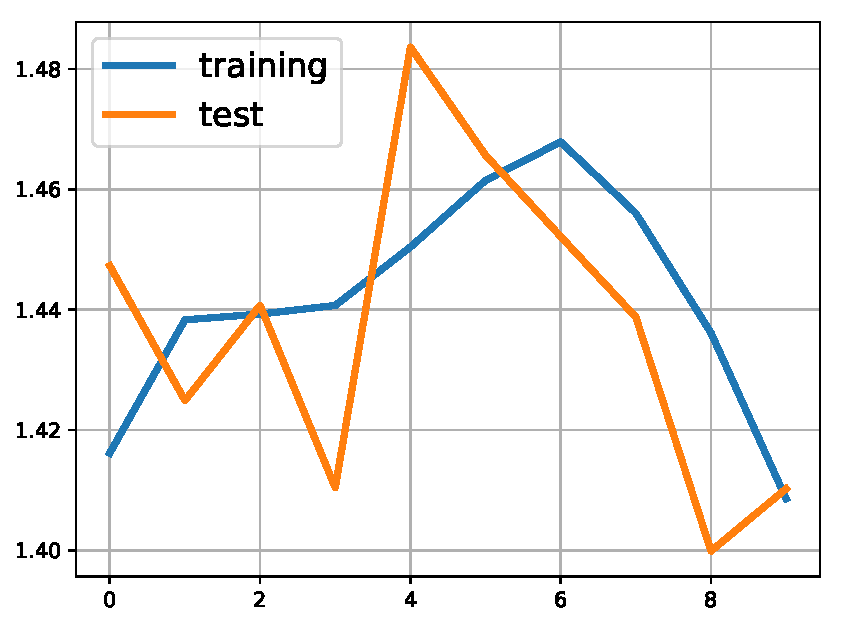
\includegraphics[width=7cm]{error.pdf} }}%
\qquad
\subfloat[confusion martix]{{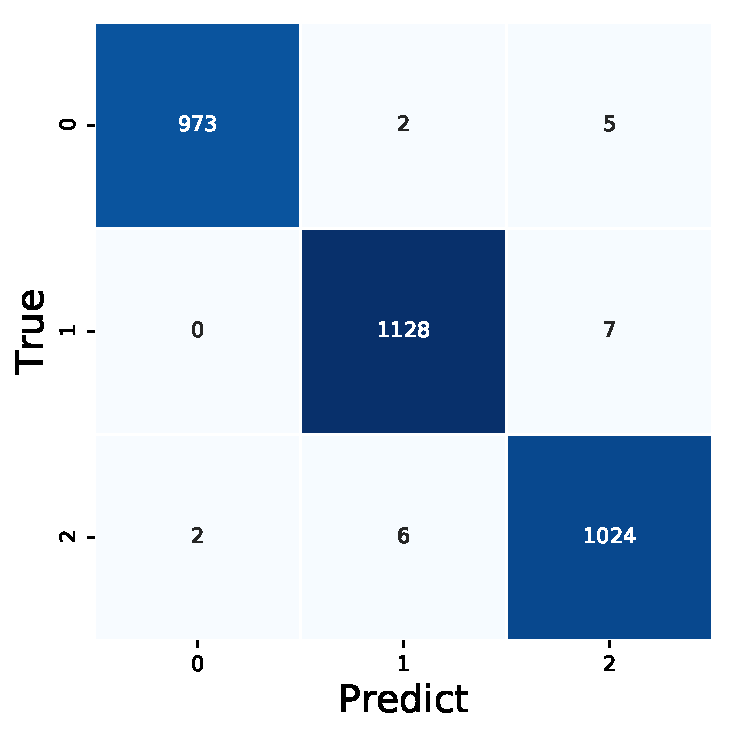
\includegraphics[width=6.5cm]{confusion.pdf} }}%
\caption{活性化関数sigmoidを用いた10エポックでの誤差関数の推移とconfusion matrix}%
\label{fig:example}%
\end{figure}

%%%%%%%%%%%%%%%%%%%%%%%%%%%%%%%%%%%%%%%%%%%%%%%%%%%%%%%%%%%%%%%%%%%%%%%%%%%
\section{考察}
以上の結果より、作成したモデルでデータのスキャン回数(epoch 数)をあげるに連れて訓練誤差と テスト誤差が減少している様子が確認できる。Epoch 数が 10 以下のとき、訓練誤差とテスト誤差が急 激に減少している様子が見えるが、epoch 数が 10 以上の時、訓練誤差とテスト誤差が徐々に減少してい る。このモデルの場合、未学習と過学習現象が見えていない。\\
confusion matrix の結果より、誤分類各ケースの中に、3を2と誤って分類されたケースが一番多い。
また、confusion matrixの結果より、このモデルの精度は98.56\%に達しているということがわかる。\\
\begin{figure}[h]
\centering
\subfloat[3を2と誤って予測された例]{{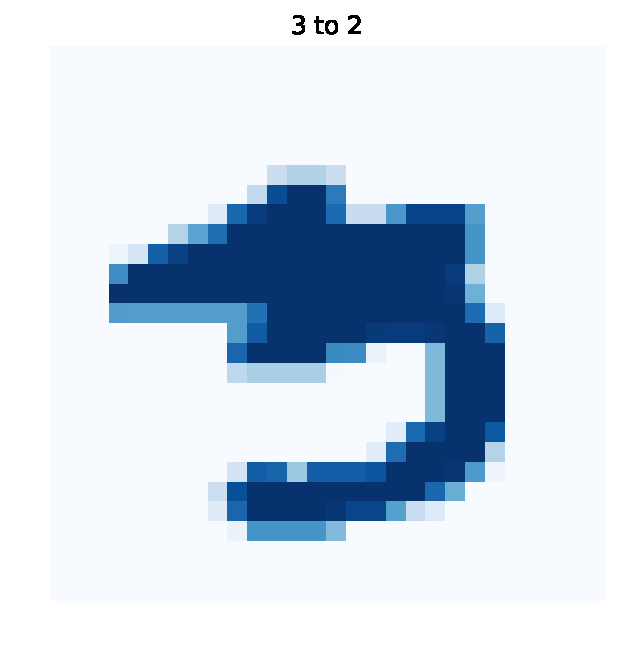
\includegraphics[width=7cm]{3to2.pdf} }}%
\qquad
\subfloat[1を2と誤って予測された例]{{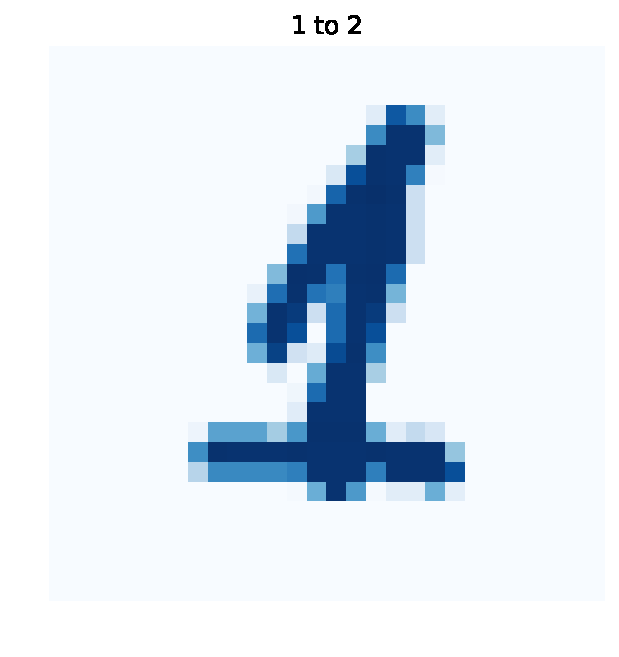
\includegraphics[width=7cm]{1to2.pdf} }}%
\caption{誤分類したデータの図示}%
\label{fig:example}%
\end{figure}


%%%%%%%%%%%%%%%%%%%%%%%%%%%%%%%%%%%%%%%%%%%%%%%%%%%%%%%%%%%%%%%%%%%%%%%%%%%
% ここまでがレポートの記述
%%%%%%%%%%%%%%%%%%%%%%%%%%%%%%%%%%%%%%%%%%%%%%%%%%%%%%%%%%%%%%%%%%%%%%%%%%%
\end{document}
